% プリアンブル
%
\documentclass[dvipdfmx]{jsarticle}
\usepackage{sty/lab_meeting}  					% 研究会資料用styファイル
\usepackage{sty/vec_and_scalar_dobashi_2011_04} % ベクトル表記用styファイル
\usepackage[dvipdfmx]{graphicx}							% 図の挿入用styファイル
\usepackage{amsmath}
\usepackage{bm} % 太字(数式)
\usepackage{subcaption} % 図表副題
\usepackage{multirow}
\usepackage{sty/cprotect}
\usepackage{enumerate} % 列挙用
\pagestyle{plain}
\newcommand{\argmin}{\mathop{\rm arg~min}\limits} %argmin
\setlength\textfloatsep{5pt}
\setlength\abovedisplayskip{5pt}
\setlength\belowdisplayskip{5pt}
\setlength\abovecaptionskip{1pt}
\setlength\fboxsep{1pt}
\setlength\fboxrule{1pt}

\begin{document}
%----------------------------------------------------
%=====================================%
% タイトル等
%=====================================%
\headding{
			2023年3月14日\\[-.25zh]
			機能ロボット学研究室\hspace{-.5zw}(MA-1)\\[-.25zh]
%			ミーティング資料
%			\hspace{-.5zw}(研究室外持出禁止) % 必要ならコメントアウトを解除
}

\title{近接点地図構築ソフトウェアの環境構築と使用方法\\[-.25zh]} % タイトル

\author{M2 和田鼓太郎} % 著者

\maketitle

%==========================================%
% 本文
%==========================================%
\section{Visual Studio Community 2019 のインストール}
QtがMSVC2019かMSVC2015としか互換性が無いようで、G2Oのインストールに必要になる.インストール方法は省略.

\section{Qt5 のインストール}
\begin{enumerate}
	\item \verb|https://www.qt.io/| でQt Account を登録
	\item \verb|https://www.qt.io/download-open-source| からオンラインインストーラをダウンロード
	\item インストーラを起動し,カスタムインストールを選択
	\item コンポーネントを選択
	\begin{enumerate}[i]
		\item 全てのチェックボックスのチェックを外す
		\item \verb|Qt| → \verb|Qt 5.15.2| → \verb|MSVC2019 64-bit| を選択
	\end{enumerate}
	\item インストール
	\item \verb|Qt/5.15.2/msvc2019_64| フォルダ内にある \verb|bin|, \verb|include|, \verb|lib|, \verb|mkspecs|, \verb|plugins| フォルダを\verb|usr/local|にコピー
\end{enumerate}

\begin{figure}[b]
	\begin{minipage}{0.50\hsize}
		\centering
		\fbox{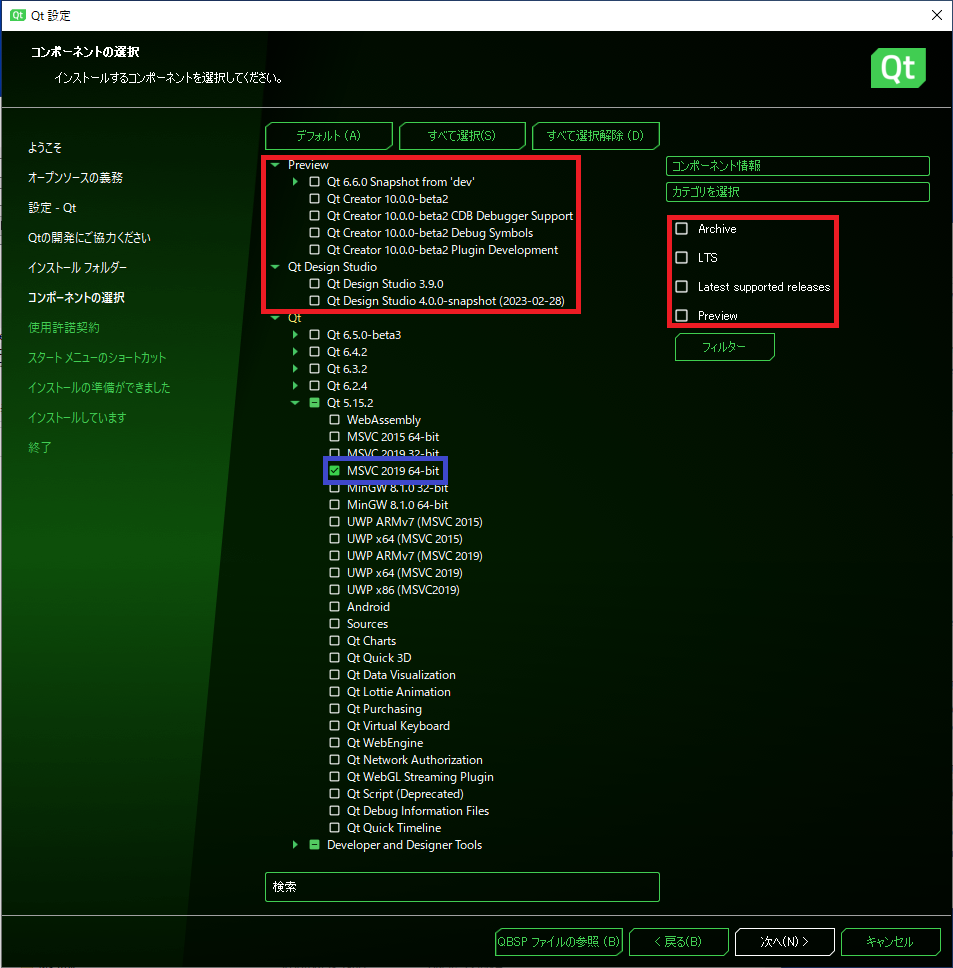
\includegraphics[height=70mm]{fig/Qt5Comp.png}}
		\subcaption{Components}
	\end{minipage}\begin{minipage}{0.50\hsize}
		\centering
		\fbox{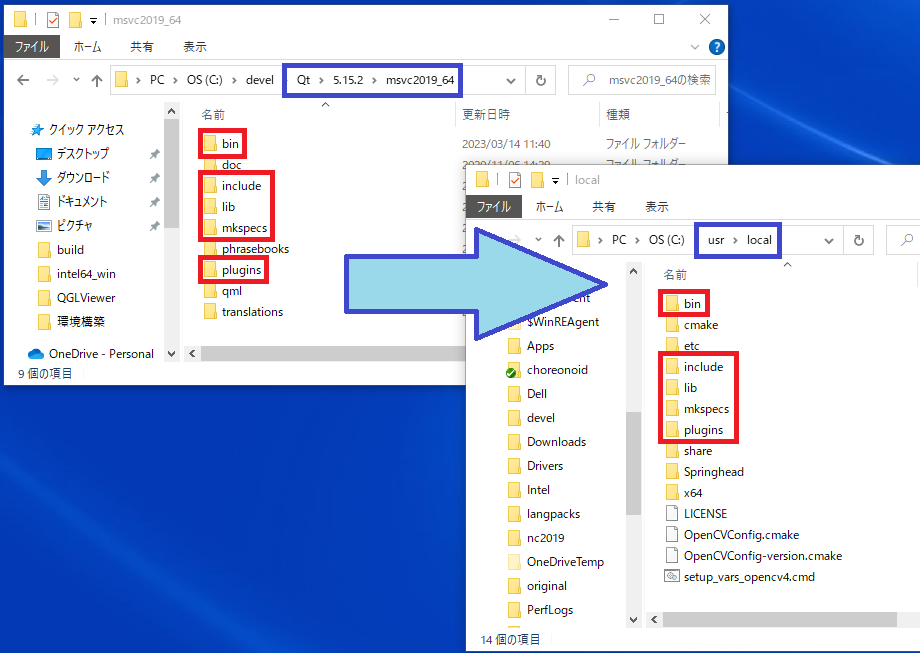
\includegraphics[height=50mm]{fig/Qt5Copy.png}}
		\subcaption{Copying}
	\end{minipage}
	\caption{Installing Qt5}
\end{figure}

\clearpage
\section{QGLViewer のインストール}
\begin{enumerate}
	\item \verb|http://libqglviewer.com/installWindows.html| からソースファイルをダウンロードし解凍
	\item Qt Creator を起動 (Qt5 と一緒にインストールされている)
	\item Qt Creator のバージョン,キットが \verb|5.15.2 MSVC2019 64bit| になっていることを確認
	\item Qt Creator で \verb|QGLViewer/QGLViewer.pro| を開く
	\item 左下のトンカチマークを押し,Debugモードでビルドを行う
	\item 左下のモニタマークを押し,Releaseモードに変更
	\item 左下のトンカチマークを押し,Releaseモードでビルドを行う
	\item Qt Creator を終了する
	\item \verb|QGLViewer| フォルダ内のヘッダファイルを \verb|usr/local/include/QGLViewer| にコピー \\
		(\verb|VRender| フォルダ内のヘッダファイルも参照関係が保たれるようにコピー)
	\item \verb|QGLViewer| フォルダ内の \verb|lib|, \verb|dll|, \verb|prl| ファイルを \verb|usr/local/lib| にコピー
	\item \verb|QGLViewer| フォルダ内の \verb|dll| ファイルを \verb|usr/local/bin| にコピー
\end{enumerate}

\begin{figure}[b]
	\begin{minipage}{0.50\hsize}
		\centering
		\fbox{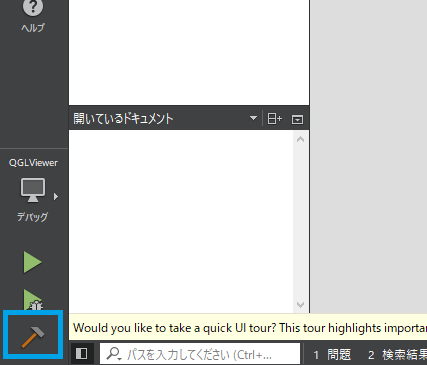
\includegraphics[height=50mm]{fig/QtBuild.png}}
		\subcaption{Debug Build}
	\end{minipage}\begin{minipage}{0.50\hsize}
		\centering
		\fbox{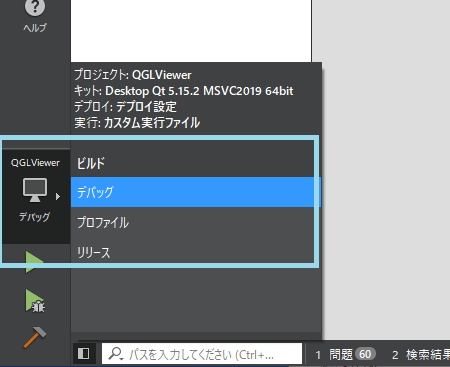
\includegraphics[height=50mm]{fig/QtRelease.png}}
		\subcaption{Changed to Release}
	\end{minipage}
	\begin{minipage}{\hsize}
		\centering
		\fbox{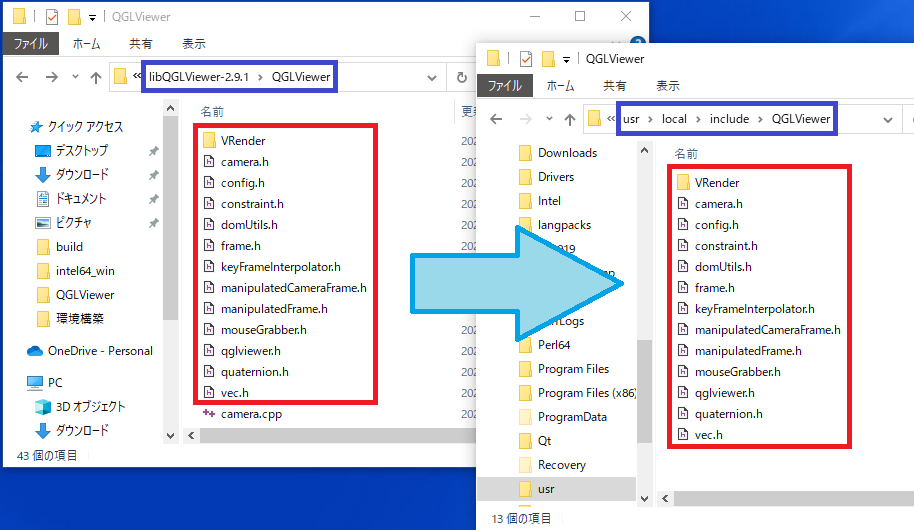
\includegraphics[height=60mm]{fig/QGLViewerCopy.png}}
		\subcaption{Copying}
	\end{minipage}
	\caption{Installing QGLViewer}
\end{figure}

\clearpage
\section{G2O のインストール}
\begin{enumerate}
	\item gitリポジトリ \verb|https://github.com/RainerKuemmerle/g2o.git| をクローン
	\item G2Oをタグ\verb|20230223_git|でチェックアウトしマージ
	\item gitリポジトリ \verb|https://github.com/WadaKotaro/prox_g2o.git| をクローン
	\item prox\_g2oのパッチ \verb|prox_g2o/0001-Pose-graph-optimization-using-Proximity-Point-Pair-m.patch| をG2Oに適用する
	\item Cmake-GuiでG2OをBuild (Cmake-Guiの使用方法は田崎先生が作成したマニュアル\verb|ソフトウェア開発環境の構築方法.pdf|を参照すること)
	\begin{itemize}
		\item \verb|CMAKE_INSTALL_PREFIX| : \verb|C:/usr/local|
		\item \verb|CMAKE_PREFIX_PATH| : \verb|C:/usr/local|
		\item エントリ \verb|G2O_BUILD_...| 系は \verb|G2O_BUILD_APPS|, \verb|G2O_BUILD_SLAM2D_TYPES| 以外不要なので,チェックを外しても良い
		\item Qt5, QGLVIEWER 関連のエントリを適切に設定
		\item SuiteSparse 関連は無視してよい (Configure中に警告を出すが無視しても正常に機能する)
	\end{itemize}
	\item Visual Studio 2019 を用いて,生成されたソリューションファイル \verb|g2o/build/g2o.sln| を Debug, Release モードで ALL\_BUILD し INSTALL
\end{enumerate}

\begin{figure}[b]
	\begin{minipage}{0.4\hsize}
		\centering
		\fbox{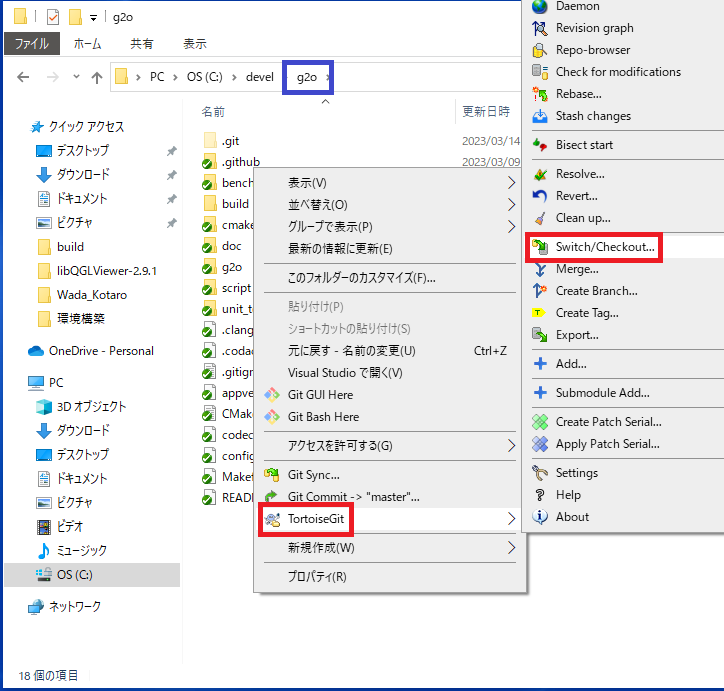
\includegraphics[height=50mm]{fig/G2OCheckout.png}}
		\subcaption{Checkout}
	\end{minipage}\begin{minipage}{0.3\hsize}
		\centering
		\fbox{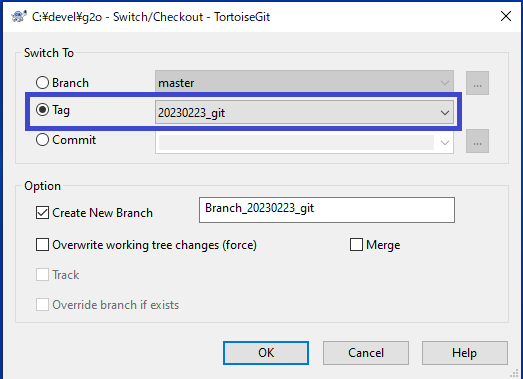
\includegraphics[height=30mm]{fig/G2OTag-20230223.png}}
		\subcaption{Tag : 20230223\_git}
	\end{minipage}\begin{minipage}{0.3\hsize}
		\centering
		\fbox{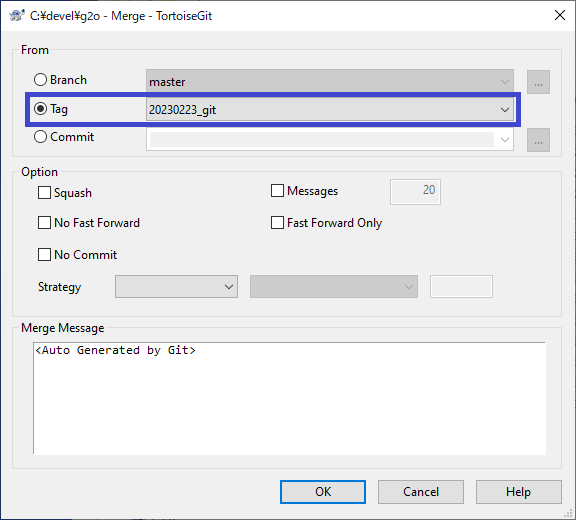
\includegraphics[height=40mm]{fig/G2OMerge.png}}
		\subcaption{Merge : 20230223\_git}
	\end{minipage}
	\caption{Checkout G2O}
\end{figure}
\begin{figure}[b]
	\begin{minipage}{0.4\hsize}
		\centering
		\fbox{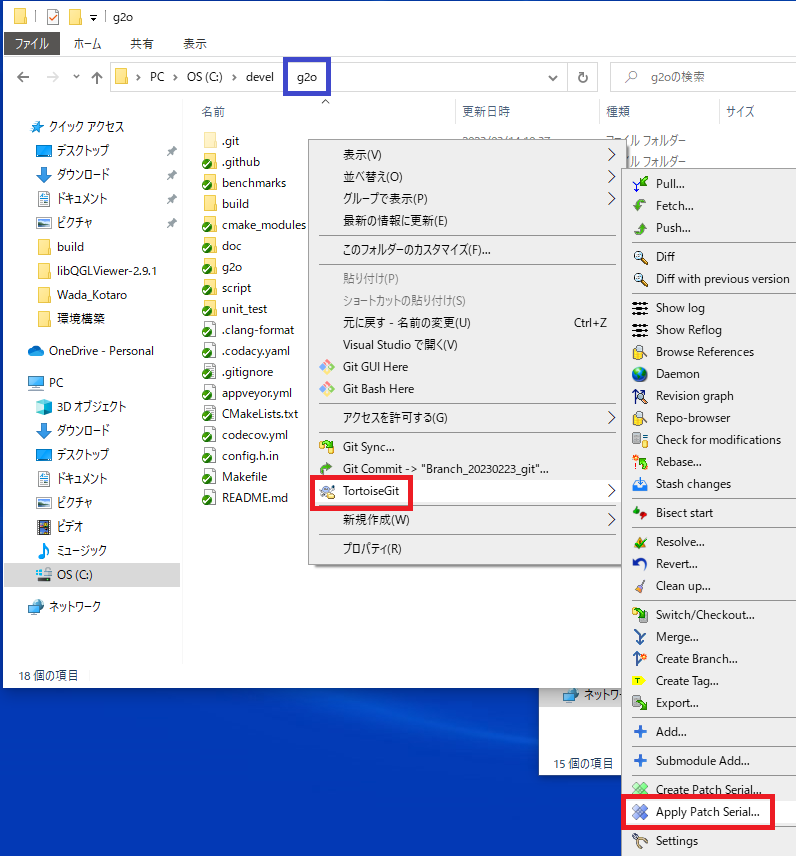
\includegraphics[height=55mm]{fig/G2OPatch.png}}
	\end{minipage}\begin{minipage}{0.6\hsize}
		\centering
		\fbox{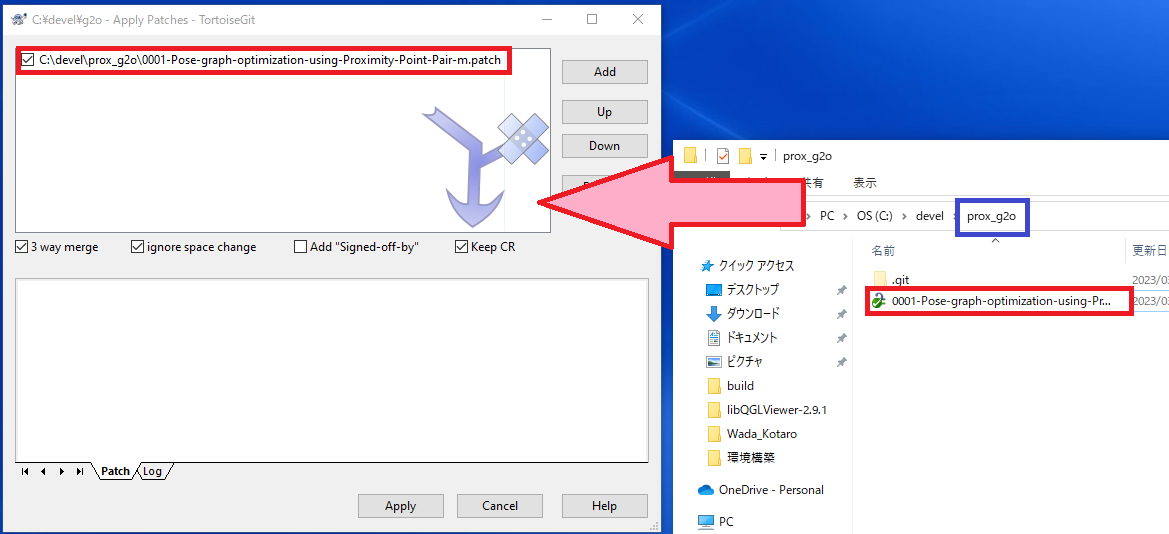
\includegraphics[height=40mm]{fig/G2OPatch2.png}}
	\end{minipage}
	\caption{Apply patch to G2O}
\end{figure}

\clearpage
\begin{figure}[t]
	\begin{minipage}{0.5\hsize}
		\centering
		\fbox{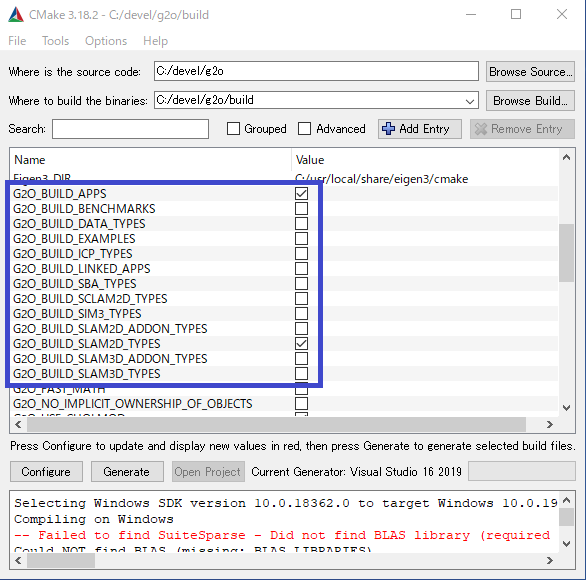
\includegraphics[height=55mm]{fig/G2OEntry.png}}
	\end{minipage}\begin{minipage}{0.5\hsize}
		\centering
		\fbox{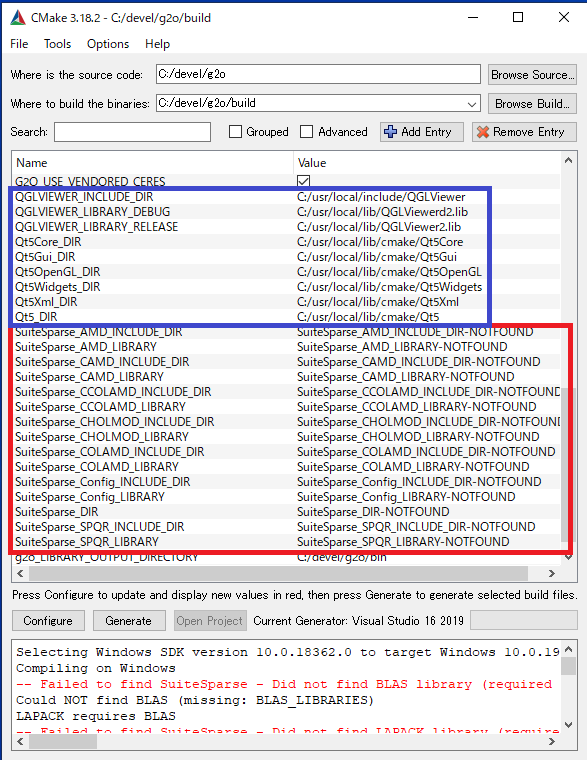
\includegraphics[height=75mm]{fig/G2OEntry2.png}}
	\end{minipage}
	\caption{Entries for build G2O}
\end{figure}

\section{MapConstructor のインストール}
\begin{enumerate}
	\item gitリポジトリ \verb|https://github.com/WadaKotaro/MapConstructor.git| をクローン
	\item Cmake-GuiでBuild
	\begin{itemize}
		\item \verb|CMAKE_INSTALL_PREFIX| : \verb|C:/usr/local|
		\item \verb|CMAKE_PREFIX_PATH| : \verb|C:/usr/local|
		\item Boost, expat, Eigen3, GLEW, GLUT(freeglut), MKL, Scenebuilder, Springhead, g2o 関連のエントリを適切に設定
	\end{itemize}
	\item Springheadのマクロ \verb|isnan| とEigen3のクラス \verb|isnan| が重複定義されエラーを出すので,Springheadの \verb|Env.h| のマクロ\verb|isnan|の定義をコメントアウトする\\
		(その場しのぎ的な策であるがMapConstructorやSystembuilder, Omniaは問題なく機能する)
	\item Visual Studio を用いて,生成されたソリューションファイル\\ \verb|MapConstructor/build/MapConstructor.sln| を Debug, Release モードで ALL\_BUILD する
	\item プロジェクト \verb|MapConstructor| をスタートアッププロジェクトに設定し F5 キーで実行することで,MapConstructorによる近接点地図の構築ができる
\end{enumerate}

\subsection{実行中に ntdll.dll にてエラー0xc0000005, 0xc0000374が発生する場合}
\begin{enumerate}
	\item Application Verifier を起動する
	\item \verb|MapConstructor/build/Release/MapConstructor.exe| を Application Verifier でテストするアプリケーションに追加し保存
	\item 再度Visual Studio で MapConstructor を実行
\end{enumerate}
ntdll.dllのエラーは何らかの理由でヒープ破損し発生していると思われる.同条件で実行しても発生しない場合があり再現性が低いため,詳細な原因は不明である.

\clearpage
\section{MapConstructor の使用方法}
Config Files のxmlファイルで実行内容を設定し F5 キーで実行する.

\cprotect \subsection{\verb|platform.xml| ファイル}
\verb|platform| タグの要素 \verb|name| を用いて実行する xml ファイルを指定する.(拡張子 .xml は書かない.) 実行するxmlファイルは \verb|MapConstructor/conf| に配置しなければ認識されないので注意.

以降に説明するタグは,実行する xml ファイルに書く.

\cprotect \subsection{\verb|SEQUENCE| タグ}
実行時に行うタスクを羅列する.タスクの指定は \verb|task| タグの要素 \verb|name| を用いて指定する.また,タスクによっては実行内容の指定が必要なものもある.実行内容の指定は要素 \verb|name| にスペース区切りで書いて指定する.(例 : タスク名 \verb|BeforePGO| の実行内容 \verb|Save| を行う場合→ \verb|<task name="BeforePGO Save"/>|) スペース区切りで実行内容を指定しているため,各タスクの \verb|name| にはスペースを使わないこと.

\cprotect \subsection{\verb|MapLoader| タグ}
Omnia を用いて生成した時系列データやループが保存された csv ファイルを読み込む.

\begin{tabular}{c|l}
	\hline
	要素 & 内容 \\
	\hline \hline
	\verb|name| & \verb|SEQUENCE| のタスク指定に用いるタスクの名前 \vspace{-5pt}\\
		& (重複しないように注意, スペースは使わないこと) \\
	\verb|mapNum|  & 読み込む時系列データの数を指定する \\
	\verb|loadFormat|  & 読み込む形式をスペース区切りで羅列する \\
	\verb|MatchFile|  & ループ (近接点対) を保存しているファイル名 \\
	\verb|PoseRefFile|  & ループ (相対ポーズ) を保存しているファイル名 \vspace{-5pt}\\
		& (MapConstructor にて生成される) \\
	\hline
\end{tabular}

\begin{itemize}
	\item \verb|Map| タグを用いて各時系列データの読み込み設定を指定する
	\item \verb|loadFormat|には \verb|Loc|, \verb|Prox|, \verb|Geo|, \verb|PC|, \verb|Movement|, \verb|Match|, \verb|PoseRef| が指定可能
\end{itemize}

\cprotect \subsubsection{\verb|Map| タグ}
\begin{tabular}{c|l}
	\hline
	要素 & 内容 \\
	\hline \hline
	\verb|ID|  & ループ検出の際に用いた時系列データID \vspace{-5pt} \\
		& (Matchファイルが時系列データを識別するのに必要) \\
	\verb|LocFile|  & 各フレームのロボットポーズを保存しているファイル名 \\
	\verb|ProxFile|  & 各フレームの近接点位置を保存しているファイル名 \\
	\verb|GeoFile|  & RTK測位結果を保存しているファイル名 \\
	\verb|PCFile|  & 各フレームの点群位置を保存しているファイル名 \\
	\verb|MovementFile|  & 各フレームのオドメトリを保存しているファイル名 \vspace{-5pt}\\
		& (MapConstructor にて生成される, \vspace{-5pt}\\
		& Omina で読み込めるMovementファイルとは形式が違うので注意) \\
	\hline
\end{tabular}

\clearpage
\cprotect \subsection{\verb|MapSaver| タグ}
時系列データやループを csv ファイルに書き出す.

\begin{tabular}{c|l}
	\hline
	要素 & 内容 \\
	\hline \hline
	\verb|name| & \verb|SEQUENCE| のタスク指定に用いるタスクの名前 \vspace{-5pt}\\
		& (重複しないように注意, スペースは使わないこと) \\
	\verb|mapNum|  & 書き出す時系列データの数を指定する \\
	\verb|saveFormat|  & 読み込む形式をスペース区切りで羅列する \\
	\verb|MatchFile|  & ループ (近接点対) を保存するファイル名 \\
	\verb|LocMatchFile|  & ループが定義されたノード対の位置を保存するファイル名 (gnuplot用) \\
	\verb|AbsProxMatchFile|  & ループが定義された近接点対の位置を保存するファイル名 (gnuplot用) \\
	\verb|PoseRefFile|  & ループ (相対ポーズ) を保存するファイル名 \\
	\hline
\end{tabular}

\begin{itemize}
	\item \verb|Map| タグを用いて各時系列データの書き出し設定を指定する
	\item \verb|loadFormat|には \verb|Loc|, \verb|Prox|, \verb|AbsProx|, \verb|Geo|, \verb|LocGeo|, \verb|Movement|, \verb|Match|, \verb|LocMatch|, \verb|AbsProxMatch|, \verb|PoseRef| が指定可能
\end{itemize}

\cprotect \subsubsection{\verb|Map| タグ}
\begin{tabular}{c|l}
	\hline
	要素 & 内容 \\
	\hline \hline
	\verb|ID|  & 書き出す時系列データのID \\
	\verb|LocFile|  & 各フレームのロボットポーズを保存するファイル名 \\
	\verb|ProxFile|  & 各フレームの近接点位置を保存するファイル名 \\
	\verb|AbsProxFile|  & 各フレームの近接点位置(絶対座標)を保存するファイル名 (gnuplot用) \\
	\verb|GeoFile|  & RTK測位結果を保存するファイル名 \\
	\verb|LocGeoFile|  & RTK測位結果(時系列データ座標系)を保存するファイル名 (gnuplot用) \\
	\verb|MovementFile|  & 各フレームのオドメトリを保存するファイル名 \\
	\hline
\end{tabular}

\clearpage
\cprotect \subsection{\verb|ToG2OConverter| タグ}
時系列データとループの情報を用いてポーズグラフを生成する.また,ポーズグラフのノードの情報を時系列データに反映する.

\begin{tabular}{c|l}
	\hline
	要素 & 内容 \\
	\hline \hline
	\verb|name| & \verb|SEQUENCE| のタスク指定に用いるタスクの名前 \vspace{-5pt}\\
		& (重複しないように注意, スペースは使わないこと) \\
	\hline
\end{tabular}

\begin{itemize}
	\item \verb|Forward|, \verb|Reverse| の2つの実行内容がある
	\begin{itemize}
		\item[] \verb|Forward| : 時系列データ, ループをポーズグラフにする
		\item[] \verb|Reverse| :  ポーズグラフのノードのポーズを時系列データに反映する
	\end{itemize}
	\item \verb|Node| タグを用いて各時系列データのノードの形式を指定する
	\item \verb|Odom| タグを用いて各時系列データのオドメトリ拘束形式を指定する
	\item \verb|Loop| タグを用いて各ループ区間のループ拘束の形式を指定する
\end{itemize}

\cprotect \subsubsection{\verb|Node| タグ}
\begin{tabular}{c|l}
	\hline
	要素 & 内容 \\
	\hline \hline
	\verb|ID| & この設定を適応させる時系列データIDを指定する \vspace{-5pt}\\
		& (指定しない場合は全ての時系列データに適応される) \\
	\verb|Tag| & ノードのタグ名を指定する \\
	\hline
\end{tabular}

\begin{itemize}
	\item \verb|Tag|には \verb|VERTEX_SE2|, \verb|VERTEX_PROX| のいずれかが指定可能
	\begin{itemize}
		\item[] \verb|VERTEX_SE2| : 2次元3自由度のポーズノード
		\item[] \verb|VERTEX_PROX| : 2次元3自由度のポーズ + 2次元近接点位置のノード
	\end{itemize}
\end{itemize}

\cprotect \subsubsection{\verb|Odom| タグ}
\begin{tabular}{c|l}
	\hline
	要素 & 内容 \\
	\hline \hline
	\verb|ID| & この設定を適応させる時系列データIDを指定する \vspace{-5pt}\\
		& (指定しない場合は全ての時系列データに適応される) \\
	\verb|Tag| & エッジのタグ名を指定する \\
	\verb|poseRef-InfoGain| & 相対ポーズの各要素の逆数に対する重み行列のゲイン \\
	\verb|infoLimit| & 重み行列の値の上限値 \\
	\hline
\end{tabular}

\begin{itemize}
	\item \verb|Tag|には \verb|EDGE_SE2| のみが指定可能
	\begin{itemize}
		\item[] \verb|EDGE_SE2| : 2次元3自由度相対ポーズによる拘束
	\end{itemize}
	\item Movement ファイルを用いてオドメトリ情報を読み込んだ場合はそのオドメトリ情報を用いる \\
		(Movement ファイルを読み込んでいない場合は連続したノード間の相対ポーズを用いてオドメトリを定義する)
\end{itemize}

\clearpage
\cprotect \subsubsection{\verb|Loop| タグ}
\begin{tabular}{c|l}
	\hline
	要素 & 内容 \\
	\hline \hline
	\verb|ID| & この設定を適応させる時系列データIDを指定する \vspace{-5pt}\\
		& (指定しない場合は全ての時系列データに適応される) \\
	\verb|Tag| & エッジのタグ名を指定する \\
	\hline
\end{tabular}

\begin{itemize}
	\item \verb|Tag|には \verb|EDGE_SE2|, \verb|EDGE_SWITCH_SE2|, \verb|EDGE_PROX|, \verb|EDGE_SWITCH_PROX|, \verb|EDGE_M_Est_PROX| のいずれかが指定可能
	\begin{itemize}
		\item[] \verb|EDGE_SE2| : 2次元3自由度相対ポーズによる拘束
		\item[] \verb|EDGE_SWITCH_SE2| : 2次元3自由度相対ポーズによる拘束 (スイッチ変数によるロバスト化)
		\item[] \verb|EDGE_PROX| : 近接点対の幾何学的特性による拘束
		\item[] \verb|EDGE_SWITCH_PROX| : 近接点対の幾何学的特性による拘束 (スイッチ変数によるロバスト化)
		\item[] \verb|EDGE_M_Est_PROX| : 近接点対の幾何学的特性による拘束 (M推定によるロバスト化)
	\end{itemize}
	\item Match ファイルを用いて近接点対情報を読み込んだ場合は \verb|EDGE_SWITCH_PROX|, \verb|EDGE_M_Est_PROX| が利用可能
	\item PoseRef ファイルを用いて相対ポーズ情報を読み込むか,Match ファイルを用いてスキャンマッチングまたは近接点対マッチングを行なった場合は \verb|EDGE_SE2|, \verb|EDGE_SWITCH_SE2| が利用可能
\end{itemize}

\verb|Tag| を \verb|EDGE_PROX|, \verb|EDGE_SWITCH_PROX|, \verb|EDGE_M_Est_PROX| にした場合,次の要素の指定が必要である.

\begin{tabular}{c|l}
	\hline
	要素 & 内容 \\
	\hline \hline
	\verb|proxSim-InfoGain| & 近接点対の類似度に対する重み行列のゲイン \vspace{-5pt}\\
		& (0未満に設定した場合,類似度に限らず負号を取り除いた一定値を重みにする) \\
	\hline
\end{tabular}\\

\verb|Tag| を \verb|EDGE_SWITCH_SE2|, \verb|EDGE_SWITCH_PROX| にした場合,次の要素の指定が必要である.

\begin{tabular}{c|l}
	\hline
	要素 & 内容 \\
	\hline \hline
	\verb|switchInfo| & 各スイッチ変数の重み付け \\
	\hline
\end{tabular}\\

\verb|Tag| を \verb|EDGE_M_Est_PROX| にした場合,次の要素の指定が必要である.

\begin{tabular}{c|l}
	\hline
	要素 & 内容 \\
	\hline \hline
	\verb|robustKernel| & $\rho$関数の種類の指定 \\
	\verb|robustKernelDelta| & $\rho$関数のパラメータの指定 \\
	\hline
\end{tabular}
\begin{itemize}
	\item \verb|robustKernel|には \verb|Huber|, \verb|GemanMcClure| 等が指定可能
\end{itemize}

\begin{tabular}{|c|ccc|}
	\hline
	 & \verb|proxSim-InfoGain| & \verb|switchInfo| & \verb|robustKernel|,\verb|robustKernelDelta| \\
	\hline
	\verb|EDGE_SE2| & $\times$ & $\times$ & $\times$ \\
	\verb|EDGE_SWITCH_SE2| & $\times$ & $\bigcirc$ & $\times$ \\
	\verb|EDGE_PROX| & $\bigcirc$ & $\times$ & $\times$ \\
	\verb|EDGE_SWITCH_PROX| & $\bigcirc$ & $\bigcirc$ & $\times$ \\
	\verb|EDGE_M_Est_PROX| & $\bigcirc$ & $\times$ & $\bigcirc$ \\
	\hline
\end{tabular}

\clearpage
\cprotect \subsection{\verb|MapOptimizer| タグ}
G2Oを用いてポーズグラフを最適化する.

\begin{tabular}{c|l}
	\hline
	要素 & 内容 \\
	\hline \hline
	\verb|name| & \verb|SEQUENCE| のタスク指定に用いるタスクの名前 \vspace{-5pt}\\
		& (重複しないように注意, スペースは使わないこと) \\
	\verb|ItrNum| & Gauss-Newton法の反復数 \vspace{-5pt}\\
		& (0に設定した場合,目的関数が十分に収束するまで (変化が$10^{-6}未満になるまで$) 反復する) \\
	\hline
\end{tabular}\\

\cprotect \subsection{\verb|G2OFileIO| タグ}
G2Oファイルの読み込み, 書き出しを行う.

\begin{tabular}{c|l}
	\hline
	要素 & 内容 \\
	\hline \hline
	\verb|name| & \verb|SEQUENCE| のタスク指定に用いるタスクの名前 \vspace{-5pt}\\
		& (重複しないように注意, スペースは使わないこと) \\
	\verb|LoadFileName| & 読み込むG2Oファイル名 \\
	\verb|SaveFileName| & 書き出すG2Oファイル名 \\
	\hline
\end{tabular}

\begin{itemize}
	\item \verb|Load|, \verb|Save| の2つの実行内容がある
	\begin{itemize}
		\item[] \verb|Load| : G2Oファイルを読み込み,ポーズグラフに反映する
		\item[] \verb|Save| :  ポーズグラフの情報をG2Oファイルとして書き出す
	\end{itemize}
\end{itemize}

\cprotect \subsection{\verb|MapDirPrepro| タグ}
ループが定義されたノード対の進行方向の情報を用いて,各時系列データの観測開始時の方向を修正する.

\begin{tabular}{c|l}
	\hline
	要素 & 内容 \\
	\hline \hline
	\verb|name| & \verb|SEQUENCE| のタスク指定に用いるタスクの名前 \vspace{-5pt}\\
		& (重複しないように注意, スペースは使わないこと) \\
	\verb|clacSimEqMethod| & 正定疎行列連立線形方程式 $\bm{A} \bm{x} = \bm{b}$ の解法 \\
	\hline
\end{tabular}

\begin{itemize}
	\item \verb|clacSimEqMethod|には \verb|LLT|, \verb|LDLT|, \verb|PartialPivLU| 等の Eigen の疎行列線形システムソルバが指定可能
\end{itemize}

\cprotect \subsection{\verb|ProxMatcher| タグ}
ループが定義されたノード対に近接点対マッチングを行ないノード間の相対ポーズを計算する.

\begin{tabular}{c|l}
	\hline
	要素 & 内容 \\
	\hline \hline
	\verb|name| & \verb|SEQUENCE| のタスク指定に用いるタスクの名前 \vspace{-5pt}\\
		& (重複しないように注意, スペースは使わないこと) \\
	\verb|clacSimEqMethod| & 正定疎行列連立線形方程式 $\bm{A} \bm{x} = \bm{b}$ の解法 \\
	\verb|maxItr| & Gauss-Newton法の最大反復数 \vspace{-5pt}\\
		& (最大反復数に達するか,目的関数が十分に収束するまで反復する) \\
	\hline
\end{tabular}

\begin{itemize}
	\item \verb|Match| タグを用いて相対ポーズを計算するループ区間を指定する
	\item \verb|clacSimEqMethod|には \verb|LLT|, \verb|LDLT|, \verb|PartialPivLU| 等の Eigen の疎行列線形システムソルバが指定可能
\end{itemize}

\cprotect \subsubsection{\verb|Match| タグ}
\begin{tabular}{c|l}
	\hline
	要素 & 内容 \\
	\hline \hline
	\verb|ID| & ループ区間のID \vspace{-5pt}\\
		& (指定しない場合,全てのループ区間に近接点対マッチングを行う) \\
	\hline
\end{tabular}

\cprotect \subsection{\verb|ScanMatcher| タグ}
ループが定義されたノード対にスキャンマッチングを行ないノード間の相対ポーズを計算する.点群の読み込みに長大な時間が必要なので注意.

\begin{tabular}{c|l}
	\hline
	要素 & 内容 \\
	\hline \hline
	\verb|name| & \verb|SEQUENCE| のタスク指定に用いるタスクの名前 \vspace{-5pt}\\
		& (重複しないように注意, スペースは使わないこと) \\
	\verb|clacSimEqMethod| & 正定疎行列連立線形方程式 $\bm{A} \bm{x} = \bm{b}$ の解法 \\
	\verb|heightRange| & マッチングに用いる点群の高さの閾値 \vspace{-5pt}\\
		& (LiDAR センサの高さは 0.8 [m] ) \\
	\verb|countSkip| & マッチングに用いる点群をこの数毎に1つになるように間引く \\
	\verb|distSkip| & マッチングに用いる点群を各点間の距離がこの数以上になるように間引く \\
	\verb|ICPItr| & ICPアルゴリズムで点群の対応付けをする回数を指定する \\
	\verb|ignoreRatio| & 外れ値除去のために無視する対応付けの割合を指定する \vspace{-5pt}\\
		& (1つ目は進行方向が同じ向きのノード対の場合,2つ目は進行方向が逆向きの場合) \\
	\verb|maxItr| & Gauss-Newton法の最大反復数 \vspace{-5pt}\\
		& (最大反復数に達するか,目的関数が十分に収束するまで反復する) \\
	\hline
\end{tabular}

\begin{itemize}
	\item \verb|Match| タグを用いて相対ポーズを計算するループ区間を指定する
	\item \verb|clacSimEqMethod|には \verb|LLT|, \verb|LDLT|, \verb|PartialPivLU| 等の Eigen の疎行列線形システムソルバが指定可能
\end{itemize}

\cprotect \subsubsection{\verb|Match| タグ}
\begin{tabular}{c|l}
	\hline
	要素 & 内容 \\
	\hline \hline
	\verb|ID| & ループ区間のID \vspace{-5pt}\\
		& (指定しない場合,全てのループ区間にスキャンマッチングを行う) \\
	\hline
\end{tabular} \\

\cprotect \subsection{gnuplot による地図データの描画}
\verb|MapConstructor/gnuplot| フォルダのテキストファイルで描画設定を行ない, \verb|plot.plt| でグラフを \verb|fig| フォルダに出力する.描画設定に用いるテキストファイルの選択は \verb|platform.txt| を用いて行う.

\clearpage
\section{G2O Viewer の使用方法}
G2Oをインストールした際に \verb|g2o_viewer.exe| というアプリケーションが一緒にダウンロードされる.これはグラフィックインターフェイスでg2oファイルを読み込み, 最適化や書き出しを行うソフトである.\\

g2oファイルを読み込み (書き出し) \vspace{-1zh}
\begin{enumerate}
	\item File タブの Load (Save) を選択
	\item 読み込む G2O ファイルを選択 \\
		 (書き出す G2O ファイル名を設定し保存) 
\end{enumerate}

ポーズグラフ最適化 \vspace{-1zh}
\begin{enumerate}
	\item \# Iterations で反復回数を設定
	\item Initial Guess を実行
	\item Optimize を実行
\end{enumerate}

描画設定の変更 \vspace{-1zh}
\begin{enumerate}
	\item View タブの Drawing Options を選択
	\item Value で点の大きさや線の太さを変更 \\
		 (色の変更はソースファイルを修正しビルドし直す必要がある) 
\end{enumerate}



\end{document}
